
\chapter{Results}
\label{sec:org89605da}

In this section the simulation results are presented.
We first show how the mapping procedure affects the general increment of error.
After that, we analyze the metrics and their correlation with the error increase.
Finally, after a regression study, we offer a way to predict the amount of errors a circuit could get depending on the its characteristics.

\section{Impact of mapping in the overall circuit error}
\label{sec:org885658c}

After the selection of benchmarks in the \url{chapter-4.org} section, we started their simulations with the simulation framework.
Not surprisingly, some of the benchmarks had very long simulations times or were even impossible to simulate in our lab servers.
Most of them with more than ten qubits.
As we mentioned before throughout this thesis, the simulation of quantum systems is computationally exhausting.
As the number of qubits or the longitude of the circuit increases, the harder would be to simulate them.
And even more in our case, that we need to run multiple simulations in a complex error model.
Therefore, as it can be seen in \ref{tab:map_selected_benchs}, we aware the low number of qubits limitation in the analysis.

\begin{table}[htbp]
\caption{Table of the selected benchmarks to be mapped. Note that the crossed ones mean that they were to}
\centering
\small
\begin{tabular}{lrrr}
\hline
Benchmark & \# qubits & \# gates & two-qubit gates (\%)\\
\hline
sf\(_{\text{274}}\) & 6 & 781 & 0.430\\
mod5adder\(_{\text{127}}\) & 6 & 555 & 0.431\\
sf\(_{\text{276}}\) & 6 & 778 & 0.432\\
4gt4\(_{\text{v0}}\)\(_{\text{72}}\) & 6 & 258 & 0.438\\
decod24\(_{\text{bdd}}\)\(_{\text{294}}\) & 6 & 73 & 0.438\\
mod10\(_{\text{176}}\) & 5 & 178 & 0.438\\
sym6\(_{\text{145}}\) & 7 & 3888 & 0.438\\
4gt12\(_{\text{v1}}\)\(_{\text{89}}\) & 6 & 228 & 0.439\\
decod24\(_{\text{enable}}\)\(_{\text{126}}\) & 6 & 338 & 0.441\\
4mod5\(_{\text{bdd}}\)\(_{\text{287}}\) & 7 & 70 & 0.443\\
mod8\(_{\text{10}}\)\(_{\text{177}}\) & 6 & 440 & 0.445\\
one\(_{\text{two}}\)\(_{\text{three}}\)\(_{\text{v1}}\)\(_{\text{99}}\) & 5 & 132 & 0.447\\
alu\(_{\text{bdd}}\)\(_{\text{288}}\) & 7 & 84 & 0.452\\
one\(_{\text{two}}\)\(_{\text{three}}\)\(_{\text{v3}}\)\(_{\text{101}}\) & 5 & 70 & 0.457\\
hwb4\(_{\text{49}}\) & 5 & 233 & 0.459\\
rd32\(_{\text{v0}}\)\(_{\text{66}}\) & 4 & 34 & 0.471\\
alu\(_{\text{v0}}\)\(_{\text{27}}\) & 5 & 36 & 0.472\\
4mod5\(_{\text{v0}}\)\(_{\text{20}}\) & 5 & 20 & 0.500\\
ham3\(_{\text{102}}\) & 3 & 20 & 0.550\\
mod5d1\(_{\text{63}}\) & 5 & 22 & 0.591\\
4gt11\(_{\text{82}}\) & 5 & 27 & 0.667\\
xor5\(_{\text{254}}\) & 6 & 7 & 0.714\\
graycode6\(_{\text{47}}\) & 6 & 5 & 1.000\\
\hline
\end{tabular}
\end{table}

\label{tab:map_selected_benchs}
[How fidelity changes after mapping]
[Describe a bit the characteristics of these benchmarks]

\begin{figure}[htbp]
\centering
\includegraphics[width=\textwidth]{figures/f_diff_bar_plot.png}
\caption{\label{fig:org047ac6b}
}
\end{figure}
In this figure we can see [explain the points htat I'm plotting and the selection of them as well as what we are trying to show]

\begin{figure}[htbp]
\centering
\includegraphics[width=\textwidth]{figures/infid_percentage_depth_before_mapping.png}
\caption{\label{fig:orgd3d0e79}
}
\end{figure}

We can inherit that the longer the circuit is before being mapped, the less impact the mapping will have over it.
In this case, even before mapped, the circuit is going to have a low fidelity or probability of success.
And after mapped, that situation does not change that much.

\section{Analysis of the mapping metrics}
\label{sec:org6cf7738}

\begin{center}
\includegraphics[width=.9\linewidth]{figures/f_ps_correlation_with_meas_error.png}
\end{center}

\begin{center}
\includegraphics[width=.9\linewidth]{figures/f_ps_correlation_no_meas_error.png}
\end{center}


\subsection{Metrics behaviour}
\label{sec:org9cbd9bb}

\begin{figure}[htbp]
\centering
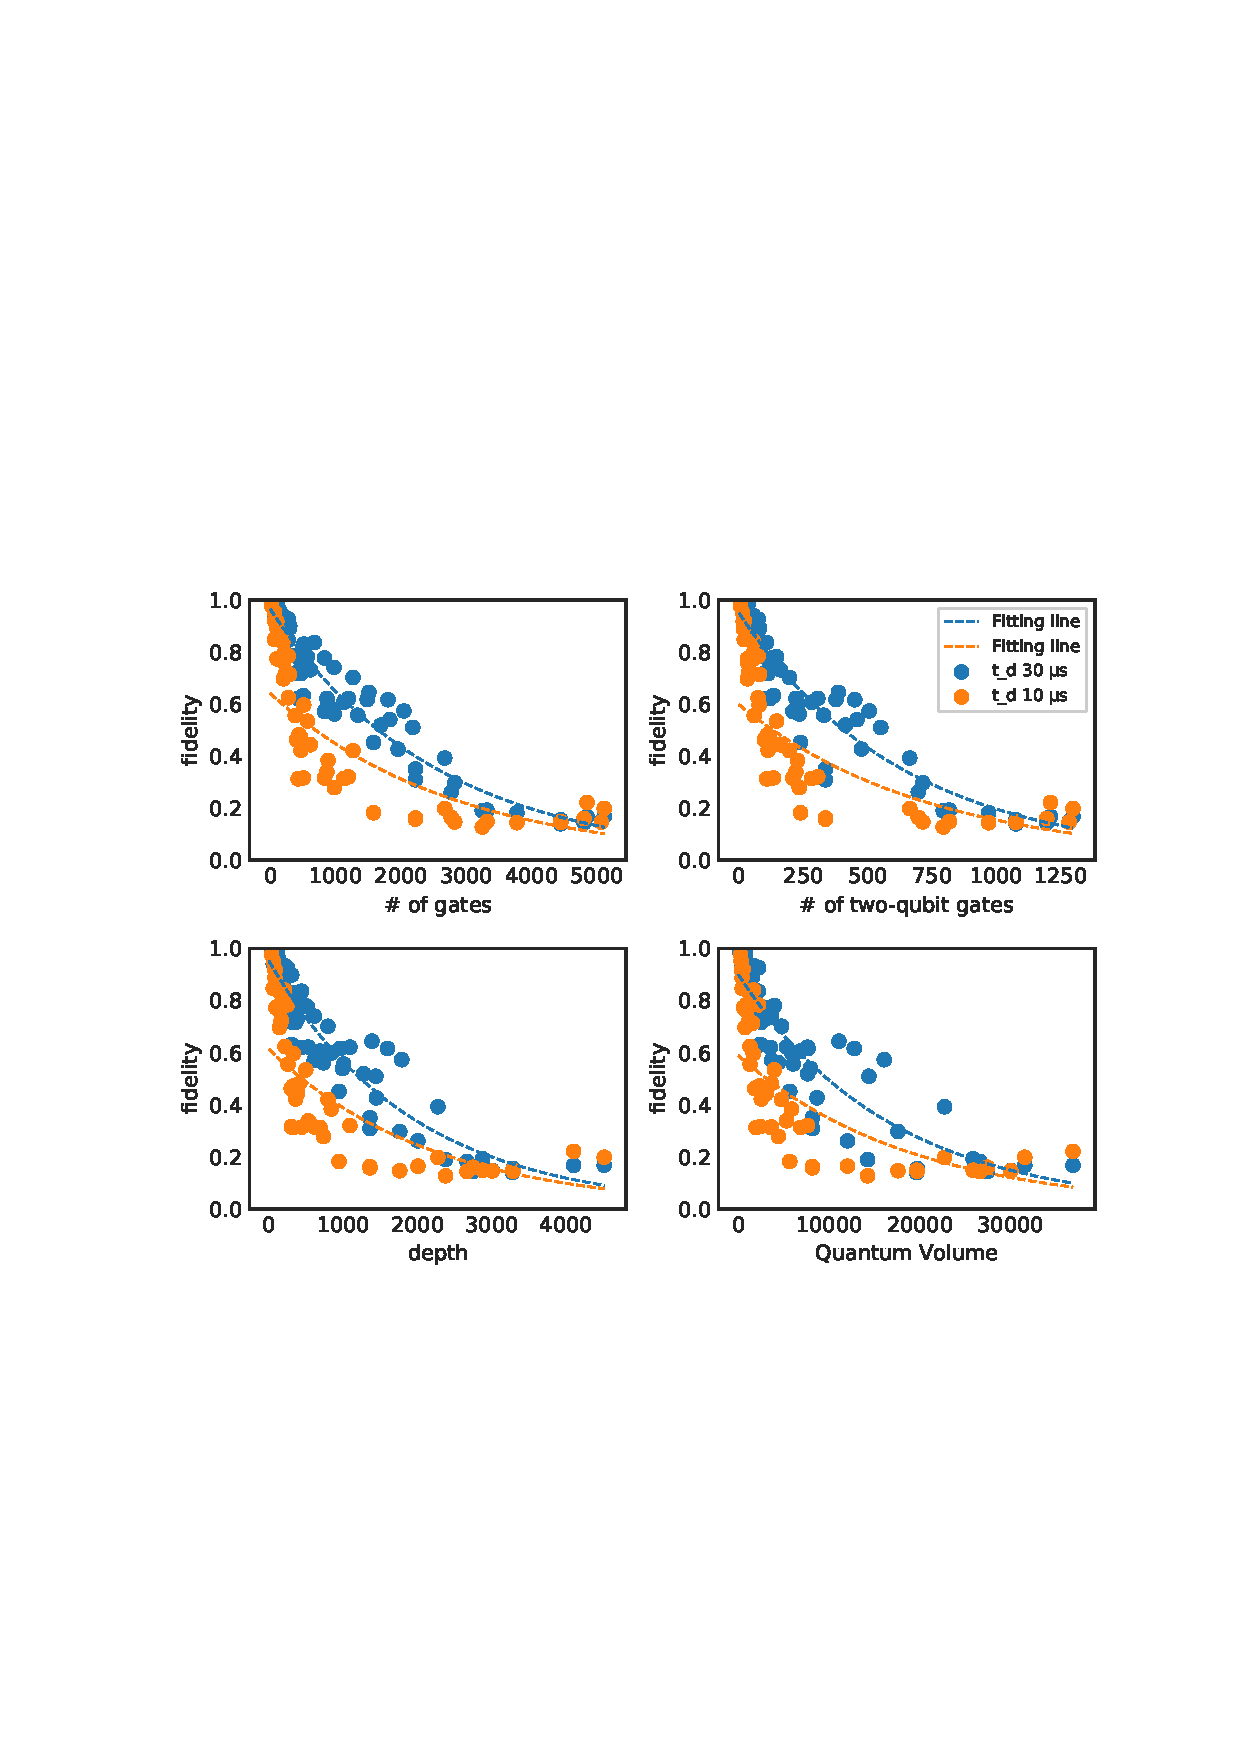
\includegraphics[width=\textwidth]{figures/f_metrics_correlation.png}
\caption{\label{fig:orgeef9ab9}
}
\end{figure}

\begin{figure}[htbp]
\centering
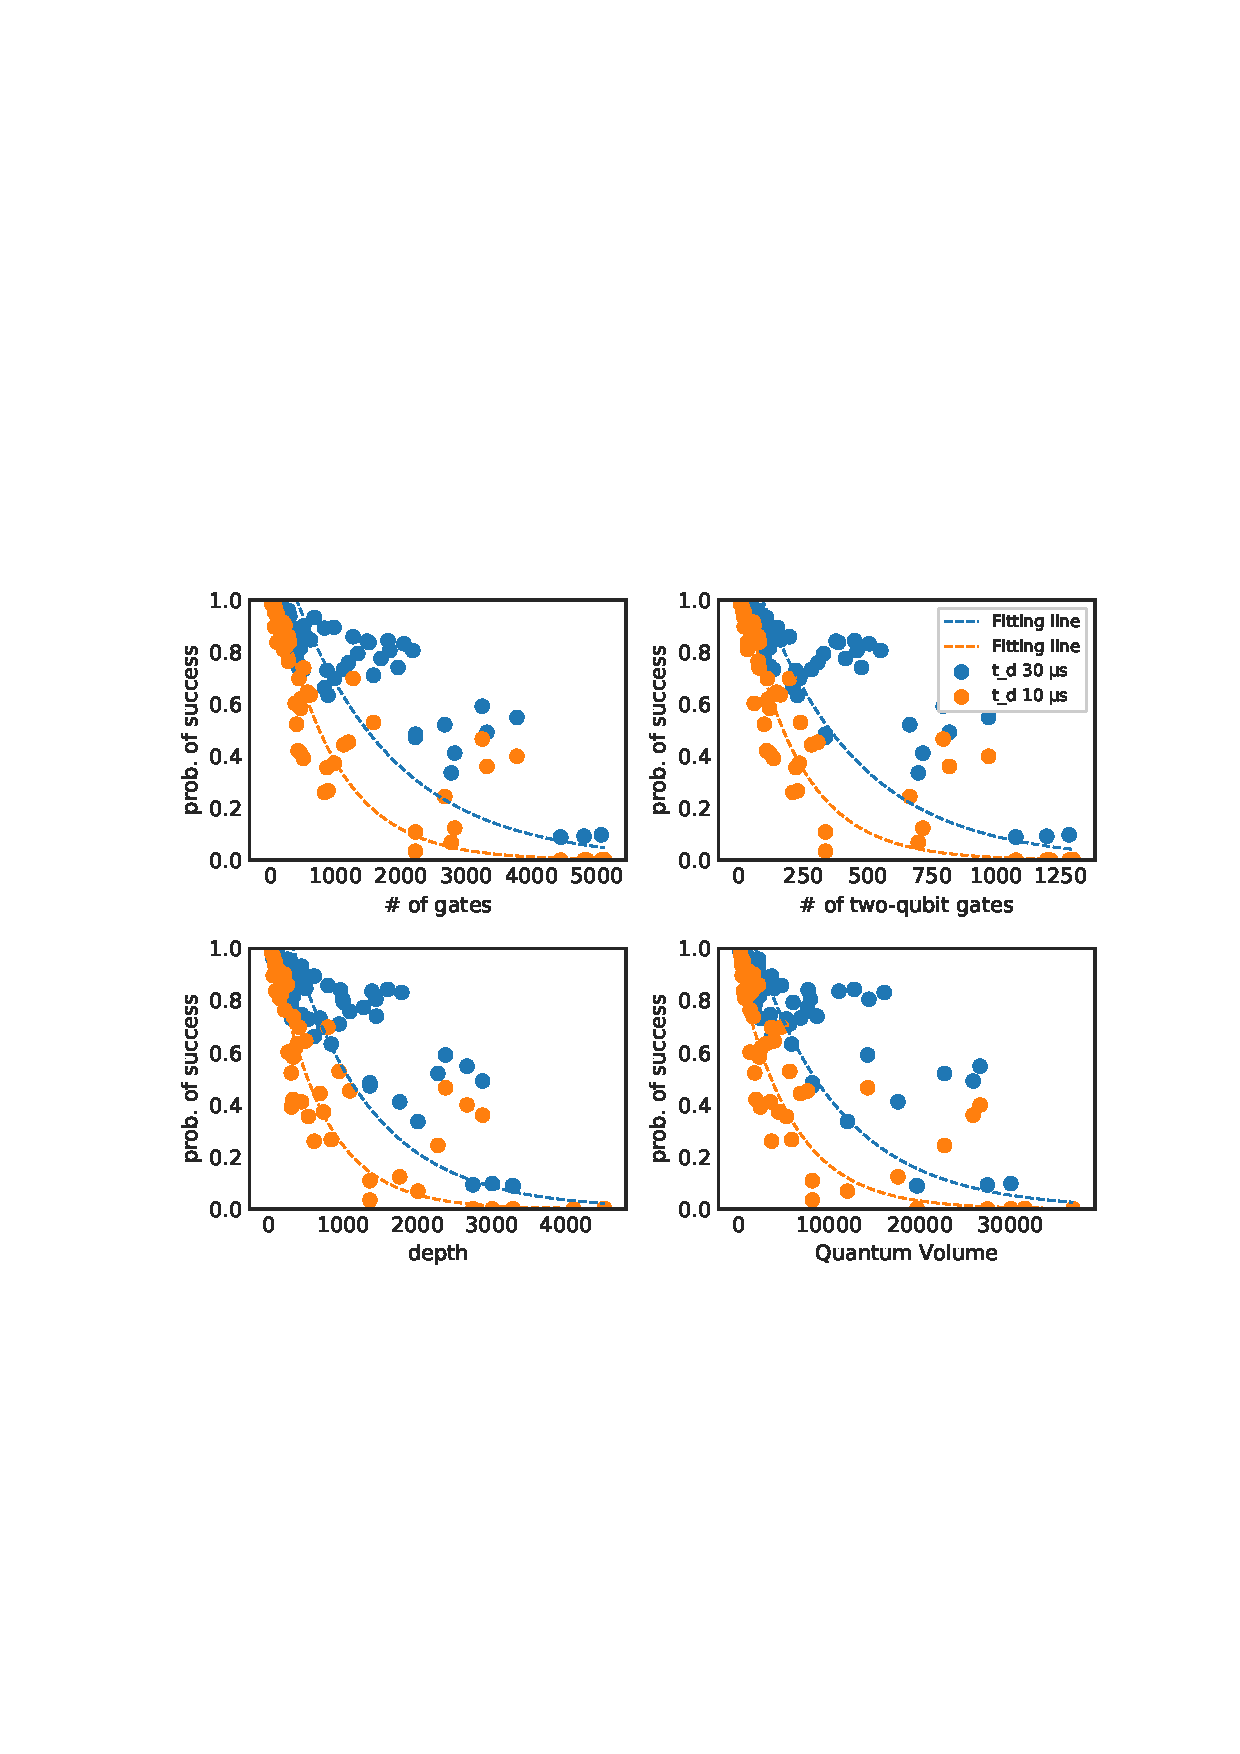
\includegraphics[width=\textwidth]{figures/ps_metrics_correlation.png}
\caption{\label{fig:orgb4b1581}
}
\end{figure}

\section{Advice}
\label{sec:org01c1deb}
